\chapter{Recifragem por \emph{Proxy}}
Nesse capítulo iremos detalhar a respeito de recifragem por \emph{proxy} (\emph{Proxy ReEncryptation} - PRE), um esquema que permite a utilização de chaves privadas de multiplos usuários para decifrar uma mensagem cifrada por um usuário \emph{u}1 sem ser necessário recifrar essa a cada vez que um usuário diferente for utilizar a mesma. Na sessão \ref{recifragem:fundamentos} irão ser apresentados os principais fundamentos da recifragem por \emph{proxy}.

% A seção \ref{recifragem:EU-PRE} irá falar sobre o \emph{Efficient Unidirectional Proxy Re-Encryption}, um esquema de recifragem por \emph{proxy} no qual é baseado a otimização proposta em \ref{recifragem:otimizacao}.


\section{Fundamentos}
\label{recifragem:fundamentos}
A recifragem por \emph{proxy} [\cite{blaze1998divertible}] é uma alternativa ao esquema criptográfico assimétrico tradicional [\cite{1363std}] que permite a delegação de direitos de acesso a messagens cifradas de maneira eficiente e mais segura. Em um cenário tradicional caso o usuário \emph{u}1 queira que somente os usuários \emph{u}2 e \emph{u}3 tenham acesso a suas mensagens cifradas ele primeiro cifra suas mensagens com sua chave privada (\emph{sk}1), em seguida cifra novamente com as chaves de \emph{u}2 e \emph{u}3 separadamente, de forma que ao distribuir essa mensagem cada um com suas respectivas chaves privadas e a chave pública de \emph{u}1 poderá decifrar a mensagem.

Em cenários onde se tem uma certa volatilidade quanto aos usuários e que a mensagem a ser transmitida não altera com tanta frequência, ou seja, existe mais mudanças de usuários que do conteúdo da mensagem. A abordagem tradicional de criptografia assimétrica se mostra uma abordagem pouco eficiente, visto que para cada vez que um usuário diferente necessitar consumir o conteúdo será necessário recifrar a mensagem a ser transmitida usando sua respectiva chave pública (\emph{pk}n) de forma que somente ele consiga reproduzi-la. Uma outra abordagem possível é através da entrega da chave privada de \emph{u}1 à \emph{u}n [\cite{ma2009group}]. Porém essa abodargem apresenta grande desvantagem visto que \emph{u}n terá acesso a chave privada de \emph{u}1 e por consequência terá acesso a todas as suas mensagens e por isso deve ser uma entidade confiável de \emph{u}1[\cite{libert2011unidirectional}].

A recifragem por \emph{proxy} explora as adptações do modelo tradicional introduzindo um novo elemento, o \emph{proxy}, que será responsável por intermediar a validação de chaves entre o usuário \emph{u}1 e seus consumidores. Simplificando é como se o \emph{proxy} agora fosse o responsável por fornecer as chaves de acesso ao conteúdo gerado por \emph{u}1 sem que o mesmo precise fornecer sua chave privada ou mesmo ter que recifrar todo o conteúdo com a chave pública dos usuários que irão consumir o mesmo.

Neste sistema o usuário \emph{u}1 irá cifrar seu conteúdo uma vez e o enviará para o \emph{proxy}. Paralelamente será gerado uma chave de recifragem que também será enviada ao \emph{proxy}. Dentro deste o conteúdo será recifrado utilizando agora a chave de recifragem de \emph{u}1 para \emph{u}n. Essa chave de recifragem permitirá ao usuário \emph{u}n decifrar o conteúdo recifrado pelo \emph{proxy} com a sua respectiva chave privada (\emph{pk}n) confome podemos observar na figura:
\begin{figure}[H]
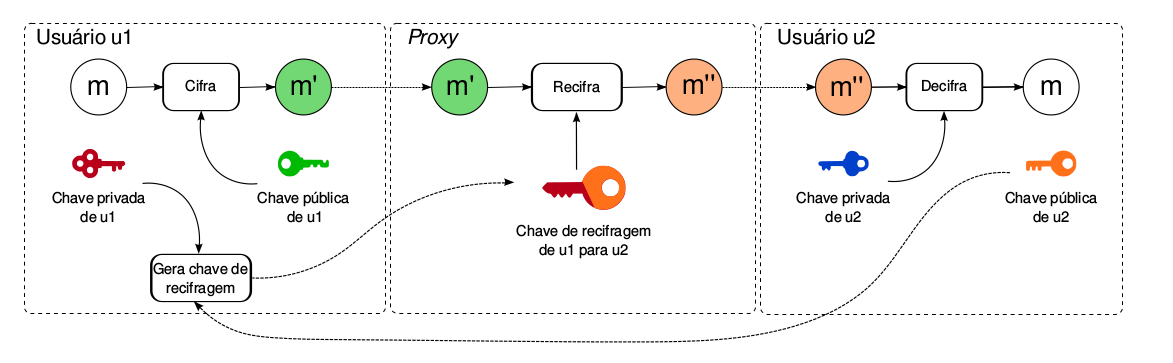
\includegraphics[width=17cm]{Figuras/recifragemPorProxy.png}
\caption{Recifragem por \emph{proxy} (\cite{mannes2016controle})} 
\label{figura:RecifragemProxy} 
\end{figure}

Há algumas premissas de operações padrão do esquemas de recifragem por \emph{proxy}. A implementação dos mesmos vai depender do tipo de recifragem[\cite{ateniese2006improved}, \cite{chow2010efficient}]:

\textbf{\textit{Configuração:}} Recebe como entrada um parâmetro de segurança $k$ e tem como saída uma tupla de parâmetros globais. 

\textbf{\textit{Geração de chaves:}} Gera os pares de chaves pública, $pk$, e privada, $sk$.

\textbf{\textit{Cifragem:}} Recebe $pk_{(u1)}$ e uma mensagem $m$, gera uma mensagem $\{m\}_{pk_{(u1)}}$.

\textbf{\textit{Geração de chave de recifragem:}} Tem como entrada a chave privada $sk_{(u1)}$ e a chave pública $pk_{(u2)}$ e como saída uma chave de recifragem $rk_{u1 \rightarrow u2}$.

\textbf{\textit{Recifragem:}} Recebe a chave de recifragem $rk_{u1 \rightarrow u2}$ e o texto cifrado $\{m\}_{pk_{(u1)}}$ , tem como saída $\{m\}_{pk_{(u2)}}$.

\textbf{\textit{Decifragem:}} Utilizando $sk_{(u2)}$ e $\{m\}_{pk_{(u2)}}$, gera como saída a mensagem $m$.

Afim de que o método seja considerado seguro foram incorporado diversas propriedades que respeitam 3 asserções básicas: (1) o \emph{proxy} não pode ser capaz de acessar o conteúdo da mensagem que recifra; (2) o usuário \emph{u}2 não pode obter o conteúdo da mensagem sem a interveção da função de recifragem; (3) O \emph{proxy} não pode, em hipótese nenhuma, obter as chaves privadas em posse das chave de recifragem e da mensagem cifrada[\cite{matsuo2007proxy},\cite{zhu2010new}].

Um resumo das possíveis caractéristicas de uma recifragem por \emph{proxy} está definido na tabela.

% ######## init table ########
%% ######## init table ########

\begin{table}[!htp]
\begin{tabular}{|c|c|c|}
\hline
Propriedades & Valores & Descrição \\ \hline
\multirow{Direção da delegação} & Unidirecional  & a  delegação $u1 \rightarrow u2$ não implica na delegação de $u2 \rightarrow u1$ \\ \cline{2-2}\cline{3-3} 
& Bidirecional  & a delegação u1 → u2 implica na delegação de u2 → u1 \\ \hline

\multirow{Número de saltos de recifragrem} & Único Salto \centering & somente mensagens originais podem ser recifradas \\ \cline{2-2}\cline{3-3} 
& Multiplos Saltos \centering & uma mensagem recifrada de u1 → u2 pode ser novamente recifrada de u2 → u3 \\ \hline

\multirow{Transitividade da chave de recifragem} & Transitivo & descrição transitivo \\ \cline{2-2}\cline{3-3} 
& Intransitivo \centering & o proxy não pode, a partir de rk u1→u2 e rk u2→u3 ,produzir rk u1→u3 \\ \hline

\multirow{Necessidade de iteração com o usuário} & Iterativo \centering & as chaves de recifragem são geradas por u1 com a necessidade de interações com u2 \\ \cline{2-2}\cline{3-3} 
& Não iterativo \centering & as chaves de recifragem são geradas por u1 sem a necessidade de interações com u2 \\ \hline

\multirow{Robustez contra conluio} & Robusto \centering & o usuário u2 e o proxy em conluio não conseguem recuperar a chave privada de u1 \\ \cline{2-2}\cline{3-3} 
& Não robusto \centering & o usuário u2 e o proxy em conluio conseguem recuperar a chave privada de u1 \\ \hline
\end{tabular}
\caption{Propriedades dos esquemas de recifragem por \textit{proxy}}
\label{table}
\end{table}

A recifragem por \emph{proxy} gerou então diversas abordagens com combinações mistas de propriedades. Dentro dessas abordagens está \emph{Efficient Unidirectional Proxy Re-Encryption} (EU-PRE) [\cite{chow2010efficient}] que contempla as seguintes propriedades: (1) \textit{Unirediconal}, (2) \textit{Único salto}, (3) \textit{Intrasitivo}, (4) \textit{Interativo} e (5) \textit{Robusto contra coluio}.

Outros duas abordagens também se encaixam nessas mesmas propriedades: são elas o esquema de \emph{proxy} invisível[\cite{jia2010cca}] e o esquema de \emph{proxy} anônimo [\cite{shao2012anonymous}]. Dessas três abordagens o EU-PRE se mostra mais simples e eficente, pois não implementa as funções de anonimato das mensagens cifradas e nem as funções de invisibilidade do \emph{proxy}.

Além disso, o trabalho de \cite{mannes2016controle} apresenta uma nova abordagem quanto ao EU-PRE. Retirando do sistema a necessidade de ter um agente de \emph{proxy}  sem impactar na segurança do processo.

Esse processo é feito através da otimização das equações matemáticas onde o processo de cifragem ainda ficará com o provedor de conteúdo e os de decifragem e recifragem ficarão a cargo do usuário. Eliminando assim um terceiro elemento do sistema, o que torna-o muito mais parecido com os que temos hoje.
%\section{\emph{Efficient Unidirectional Proxy Re-Encryptation}}
\label{recifragem:EU-PRE}
O \emph{Efficient Unidirectional Proxy Re-Encryptation}, o qual a partir daqui o iremos referenciá-lo com EU-PRE, possui seis algoritmos principais: \emph{configuração},\emph{geração de chaves}, \emph{cifragem},\emph{geração de chave de recifragem}, \emph{recifragem} e \emph{decifragem}. Que são detalhados, segundo \cite{mannes2016controle}, como os seguintes:

\paragraph{Configuração:} escolher dois números primos \emph{p} e \emph{q} tal que \emph{q} | \emph{p} - 1 (\emph{q} deve ser divisor de (p-1)), o parâmetro $\ell_0$ para o tamanho da mensagem, o parâmetro de segurança $\ell_1$ e um gerador \emph{g} do grupo $\mathbb{G}$ (um subgrupo de $\mathbb{Z^*_q}$ de ordem $q$). Além desses parâmetros, o sistema utiliza quatro funções de $hash$:$H_1 : {\left\{0,1\right\}}^{\ell_0} \times {\left\{0,1\right\}}^{\ell_1} \rightarrow \mathbb{Z^*_q}$, $H_2: \mathbb{G} \rightarrow {\left\{0,1\right\}}^{\ell_0 + \ell_1}$, $H_3 : {\left\{0,1\right\}}^{*} \rightarrow \mathbb{Z^*_q}$, $H_4 :  \mathbb{G} \rightarrow \mathbb{Z^*_q}$ . Os parâmetros públicos do sistema são: $\left(\emph{q},\mathbb{G},\emph{g},H_1,H_2,H_3,H_4,\ell_0,\ell_1\right)$.

\paragraph{Geração de chaves:} O conjunto de chaves do EU-PRE é composto por dois pares de chaves públicas-privadas para cada usuário do sistema. Essa caracaterística é introduzida por \cite{chow2010efficient} para garantir que a chave privada de um usuário \emph{u}1 não seja divulgada caso o \emph{proxy} e o usuário troquem informações. Considerando um usuário \emph{u}1, as chaves privadas $\emph{sk}1_{(\emph{u}1)}$ e $\emph{sk}2_{(\emph{u}1)}$ são escolhidas aleatoriamente em $\mathbb{Z}^*_q$ e as chaves públicas são calculadas por $\emph{g}^{sk}$, assim $sk1_{\emph({u}1)}$ = $\emph{g}^{sk_{(\emph{u}1)}}\mod{p}$ e $pk2_{(u1)} = \emph{g}^{(sk1)}\mod{p}$.   

\paragraph{Cifragem:} uma mensagem $m$ é cifrada pelo usuário $u1$
com suas chaves públicas $pk1_{(u1)}$ e $pk2_{(u1)}$. Escolher $t$ a partir de $\mathbb{Z}^*_q$ e $\omega$ de tamanho $\ell_1$ e calcular $r = H_1(m,\omega)$ e $D,E$ e $F$ como segue:
\begin{equation}
    D = ({{pk1^{H_{4(pk2_{u1})}}_{(u1)}} \times pk2_{(u1)})}^t \mod{p} )
\end{equation}
\begin{equation}
    E = ({pk1^{H_{4(pk2_{(u1)})}} \times pk2_{u1} })^r\mod{p})
\end{equation}
\begin{equation}
    F = H_2(g^r\mod{p})\oplus(m\parallel \omega) 
\end{equation}

Calcular também $ r = t+r\bullet H_3(D,E,F)\mod{p}$. A saída é $(D,F,E,s)$
\paragraph{Geração de chaves de recifragem:} Para geração de chave de recifragem de $u1$ para $u2$, são necessárias as chaves privadas de $u1$ e uma das chaves públicas de $u2$,$pk2_{(u2)}$. Deve-se escolher aleatoriamente $h$ de tamanho $\ell_0$ e $\pi$ de tamanho $\ell_1$ e calcular $v = H_1(h \times \pi)$. Calcular também $V = pk2^v_{(u2)} \mod{p}$ e $W = H_2(g^v\mod{p})\oplus(h \parallel \pi)$.
A chave de recifragem é:
\begin{equation}
    rk_{u1\rightarrow u2} = \big( {(sk1_{(u1)}) \bullet H_4(pk2_{(u2)} + sk2_{(u2)})}^{-1} \mod{p-1}  \big)
\end{equation}
A saída é $(rk_{u1\rightarrow u2},V,W)$.

\paragraph{Recifragem:}
Primeiramente o \emph{proxy} deve verificar :
\begin{equation}
\label{equation:rk}
    {(pk1^{H4(pk2_{(u1)})}_{(u1)} \bullet {pk2_{(u1)}\mod{p}})}^s \mod{p} = D \bullet (E^{H_3(D,E,F)} \mod{p} )\mod{p}
\end{equation}
E caso a equação \ref{equation:rk} seja verdadeira:
\begin{equation}
\label{equation:eu-pre:recifragem}
    E' = E^{rk_{u1\rightarrow u2}} \mod{p}
\end{equation}
A saída será $(E',F,V,W)$.
\paragraph{Decifragem:} A mensagem $m$ é decifrada por $u2$ mediante sua chave privada $sk2_{(u2)}$.
Primeiramente o usuário $u2$ recupera $(h\parallel\pi)$ e $(m\parallel\omega)$ ao calcular:
\begin{equation}
    (h\parallel\pi) = W \oplus H_2(V^{sk^{-1}_{(u2)}\mod{p-1}} \mod{p})
\end{equation}
\begin{equation}
\label{equation:eu-pre:decifragem}
    (m\parallel\omega) = F \oplus H_2(E'^{h^{-1}\mod{p-1}} \mod{p})
\end{equation}
A saída é a mensagem $m$ se $V = {pk2^{H_1(h,\pi)}_{(u2)}} \mod{p}$ e $E' = g^{H_1(m,\omega)\bullet h} \mod{p}$.
Na figura \ref{figura:fluxo_eu-pre} podemos visualizar todo o processo de recifragem do EU-PRE e o fluxo sequencial de cada etapa.
\begin{figure}[H]
\caption{Fluxo de processos do EU-PRE (\cite{mannes2016controle})
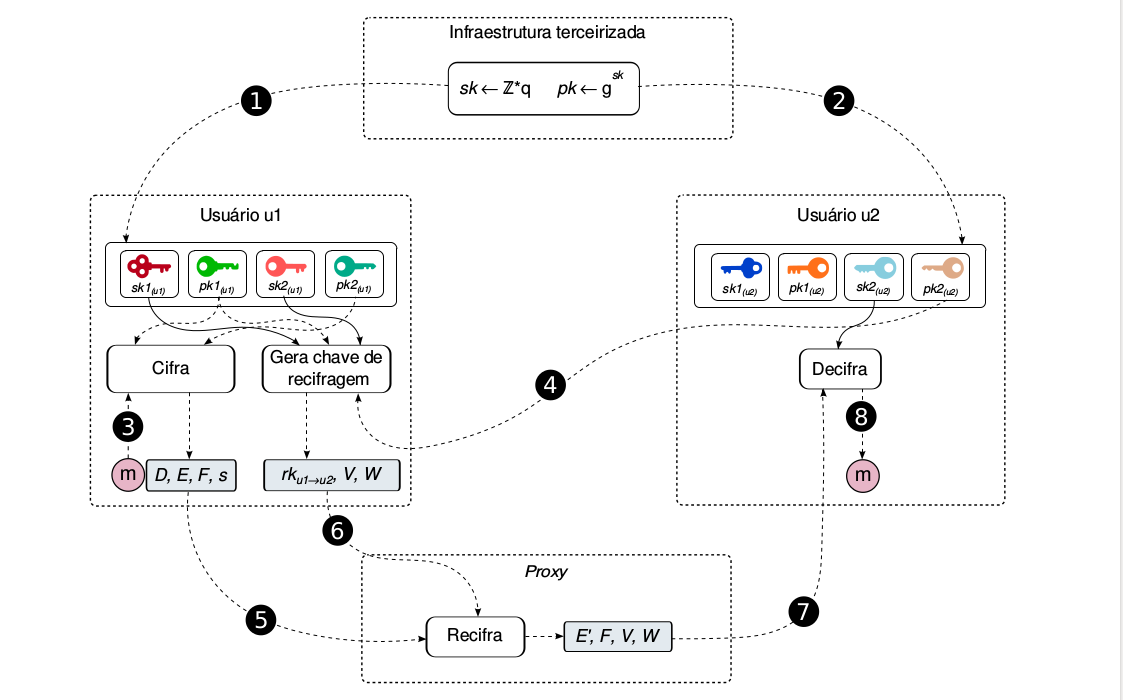
\includegraphics[height=11cm]{Figuras/fluxo_EU-PRE.png} 
\label{figura:fluxo_eu-pre}
\end{figure}

É importante salientar que no esquema de recifragrem por \emph{proxy} tradicionalmente é composto por quatro entidades: uma infraestrutura terceirizada responsável por delegar as chaves que serão utilizadas, o usuário que as delega, o \emph{proxy} e o usuário que recebe e delegação. 
Dentro desse ecosistema a divisão: Os algoritmos de configuração e geração de chaves dos usuários são executados na infraestrutura terceirizada. A cifragem e a geração de chaves de cifragem são realizadas no usuário que delega os direitos de recifragem. A recifragem é responsabilidade do \emph{proxy} e a decifragem é executada no usuário (dispositivo) que irá consumir as informações.
%\section{Otimização do \textbf{EU-PRE}}
\label{recifragem:otimizacao}
No trabalho de \cite{mannes2016controle} propõe-se uma otimização do processo do EU-PRE (\ref{recifragem:EU-PRE}). A otimizição envolve as equações \ref{equation:eu-pre:recifragem}(Recifragem) e \ref{equation:eu-pre:decifragem}(Decifragem). No modelo tradicional o \emph{proxy} recebe do provedor as variáveis $(D,E,F,s)$ e a chave de recifragem $(rk_{c\rightarrow u},V,W)$ do conteúdo $c$ para o usuário $u$. E, após a validação com as variáveis $D$ e $E$ é inciado o processo de recifragem para o $u$ através da equação \ref{equation:eu-pre:decifra}.E assim, o \emph{proxy} envia ao usuário $u$ as informações $(E',F,V,W)$ onde $E'$ é a variável calculada na equação anterior. E assim, como visto na equação \ref{equation:eu-pre:recuperaConteudo}, recupera o conteúdo cifrado pelo provedor.
\begin{equation}
\label{equation:eu-pre:decifra}
    E' = E^{rk_{c\rightarrow u}}\mod{p}
\end{equation}
\begin{equation}
\label{equation:eu-pre:recuperaConteudo}
    (m\parallel \omega) = F \oplus H_2({E'}^{h^{-1}\mod{p-1}} \mod{p})
\end{equation}
No trabalho é apresentado uma proposta de que essas duas operações sejam realizadas na mesma entidade, simplificando assim o processo de recifragem. Onde o usuário recebe o conteúdo diretamente do provedor. Essa operação é feita aplicando a variável $E$ diretamente na equação \ref{equation:eu-pre:decifra}. Eliminando a equação \ref{equation:eu-pre:decifra} ao substituir o $E'$ recebido do \emph{proxy}. Como podemos ver em \ref{equation:eu-pre:otimizacao}.
\begin{equation} \label{equation:eu-pre:otimizacao}
    \begin{split}
        (m\parallel \omega) & = F \oplus H_2({({E}^{rk_{c\rightarrow u}})^{\frac{1}{h}\mod{p-1}}} \mod{p}) \\
 & = F \oplus H_2({({E}^{rk_{c\rightarrow u{\frac{1}{h}\mod{p-1}}}})} \mod{p}) \\
 & = F \oplus H_2({({E}^{{\frac{rk_{c\rightarrow u}}{h}\mod{p-1}}})} \mod{p})
    \end{split}
\end{equation}

Com a equação final visualizada em \ref{equation:eu-pre:otimizacao} podemos ter um processo de recifragem por \emph{proxy} que possui no máximo o envolvimento de três entidades: o usuário, o provedor e uma infraestrutura responsável por delegar as chaves.

A infraestura responsável por delegar as chaves pode ainda ser substituída/rodada no provedor do conteúdo simplificando ainda mais as entidades envolvidas para duas: o provedor e o usuário consumidor.


\section{Considerações Finais}

Nesse capítulo vimos por linhas gerais o esquema de criptografia conhecido como recifragem por \emph{proxy}. Vimos também um método de otimização do mesmo que possibilita a retirada do servidor de \emph{proxy} sem perder a segurança e a característica principal do processo que é permitir que o conteúdo seja cifrado uma vez por $u1$ e decifrado por $n$ usuários sem que o mesmo tenha que cifrar novamente para esses $n$ usuários com suas respectivas chaves.

Toda essa proposta pode se encaixar dentro de um ambiente de CDN. Facilitando que o conteúdo seja retrasmitido pela rede, ficando em vários servidores de ponta e estejam devidamente criptografados. E mesmo que essa base de usuários mude,como é o caso de fornecedoras de VOD, esse conteúdo não precisa ser novamente recifrado.